% arara: pdflatex
% arara: indent
% arara: indent: {overwrite: yes}
% arara: indent: {output: jeopardy_Game2.tex}
% arara: indent: {silent: yes}
% arara: indent: {trace: yes}
% arara: indent: {localSettings: yes}
% arara: indent: {onlyDefault: on}
% arara: indent: { cruft: /home/camminady/.latexindent }

\documentclass{beamer}
\usepackage{tcolorbox}
\usepackage{ocgx}
\usepackage{graphicx}
\usepackage{commands}
\usepackage{algorithm,algorithmic}
\usepackage{animate}

\setbeamertemplate{navigation symbols}{}
\setbeamersize{text margin left=0cm, text margin right=0cm}
\tcbuselibrary{skins}

% Define the Categories here !!!!!!!
\def \firstcat {\textbf{Space}}
\def \secondcat {\textbf{Aachen}}
\def \thirdcat {\textbf{Code}}
\def \fourthcat {\textbf{The Force}}
\def \fifthcat {\textbf{Numbers}}

% Define the picture for the DOUBLE Bonus here !!!
\def \doublepic {
\includegraphics[scale=0.7]{../jeopardypics/Double_Jeopardy.png}}


%%%%%%%%%%%%%%%%%%%%%%%%%%%%%%%%%%%%%%%%%%%%%%%%%%%%%%%%%%%%%%%%%%%%%%%%%%%%%%%
%%%%%%%%%%%%%%%%%%%%%%%%%%%%%%%%%%%%%%%%%%%%%%%%%%%%%%%%%%%%%%%%%%%%%%%%%%%%%%%
\begin{document}
%%%%%%%%%%%%%%%%%%%%%%%%%%%%%%%%%%%%%%%%%%%%%%%%%%%%%%%%%%%%%%%%%%%%%%%%%%%%%%%
	
% Set up the HOME slide
\begin{frame}
	\hypertarget{home}{}
	\vspace*{-.5cm}
	\subjects{\firstcat}{\secondcat}{\thirdcat}{\fourthcat}{\fifthcat}
	\prizes
\end{frame}
	
	
%%%%%%%%%%%%%%%%%%%%%%%%%%%%%%%%%%%%%%%%%%%%%%%%%%%%%%%%%%%%%%%%%%%%%%%%%%%%%
% Category 1
%%%%%%%%%%%%%%%%%%%%%%%%%%%%%%%%%%%%%%%%%%%%%%%%%%%%%%%%%%%%%%%%%%%%%%%%%%%%%
\content                       
{s1-100}                     
{\firstcat}                          
{100}{    
	\begin{textarea}[]
		\only<1>{
			After Armstrong, this man was the second person to walk on the moon.
		}
		\only<2>{
			Who is Buzz Aldrin?
		}
	\end{textarea}   
}
	
	
\content                       
{s1-200}                     
{\firstcat}                          
{200}{    
	\begin{textarea}[]
		\only<1>{
			\begin{columns}[c]
				\column{.3\textwidth}
				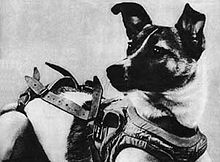
\includegraphics[height=1.0\linewidth]{../categories/media/space/laika.jpg}
				\column{.3\textwidth}	
				This soviet dog became one of the first animals in space.
			\end{columns}
																
		}
		\only<2>{
			Who is Laika?
		}
	\end{textarea}           
}
	
	
\content           
{s1-300}                     
{\firstcat}                          
{300}{                       
	\begin{textarea}[]
		\only<1>{
			\begin{columns}[c]
				\column{.3\textwidth}
				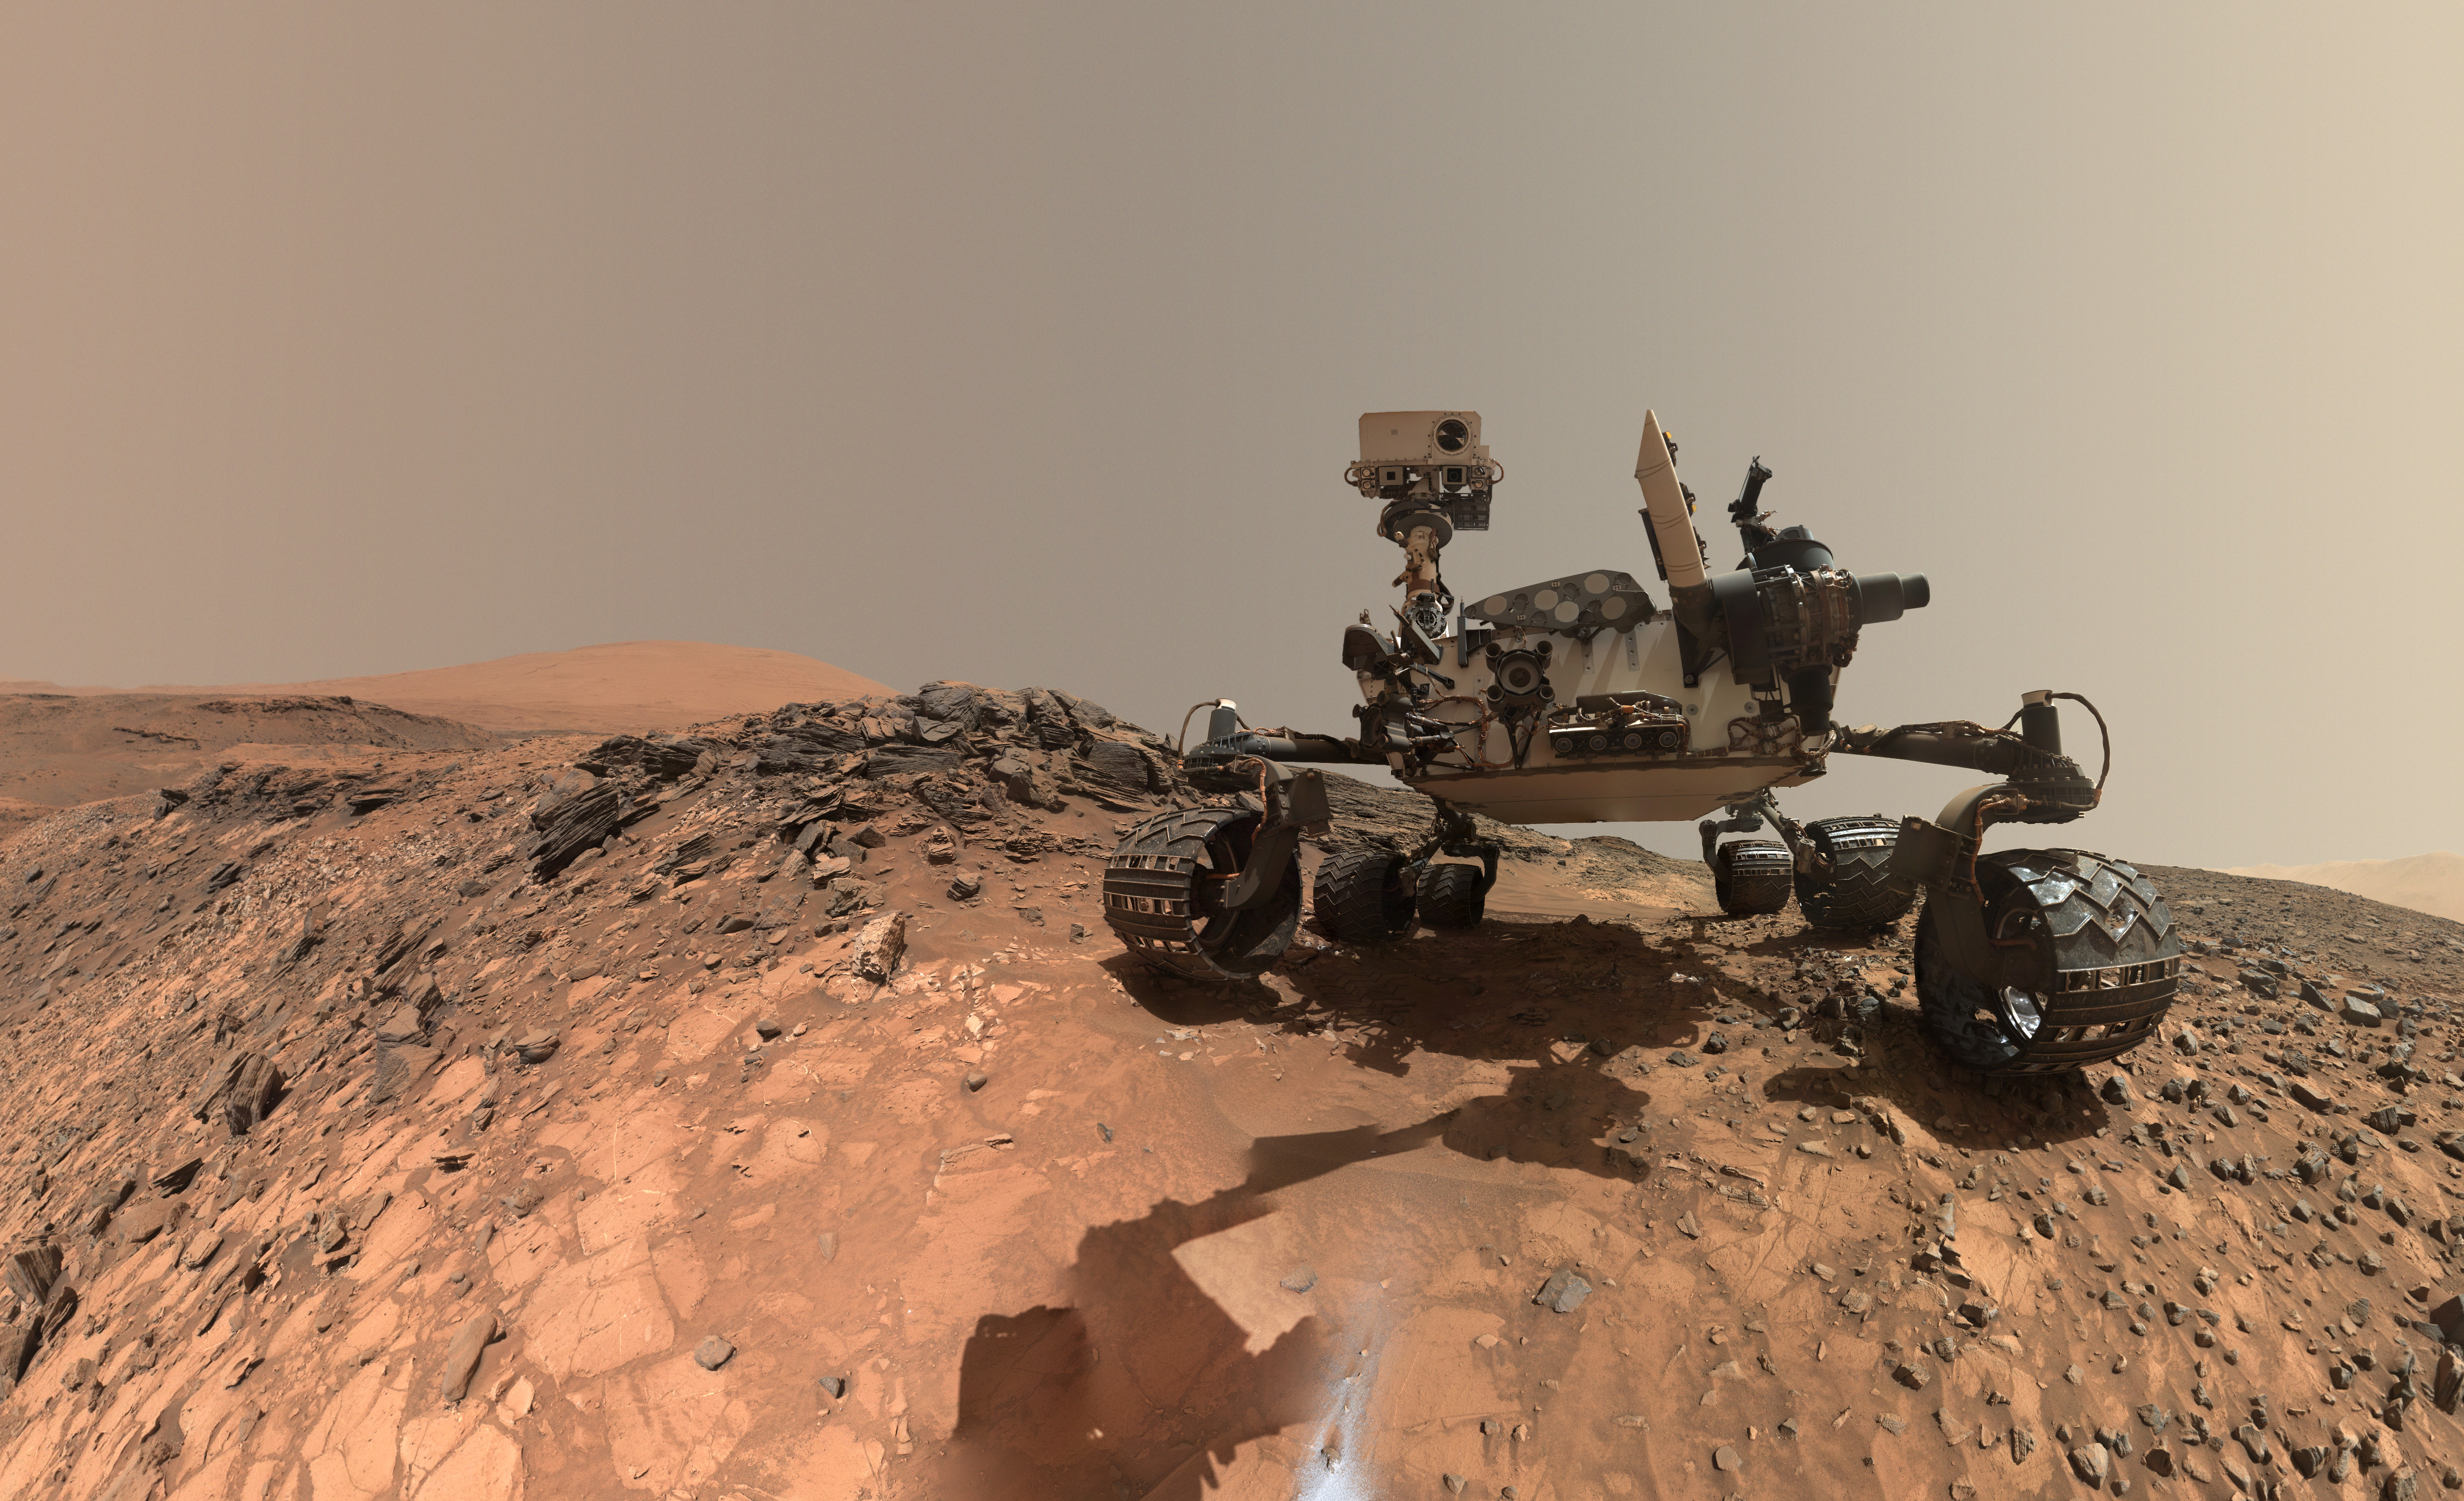
\includegraphics[height=.7\linewidth]{../categories/media/space/selfie.jpg}
				\column{.3\textwidth}	
				It took quite some effort to take a selfie of this guy.
			\end{columns}
		}
		\only<2>{
			What is the Curiosity Rover?
		}
	\end{textarea}
}
	
	
\content                       
{s1-400}                     
{\firstcat}                          
{400}{    
	\begin{textarea}[]
		\only<1>{
			In 2003, this space shuttle reentry ended in a disaster due to parts of the insulation breaking off.
		}
		\only<2>{
			What is the Space Shuttle Columbia?
		}
	\end{textarea}   
}
	
	
\content                       
{s1-500}                     
{\firstcat}                          
{500}{    
	\begin{textarea}[]
		\only<1>{
			Founded by the Tesla Motors CEO, this company achieved the first vertical landing of a first stage.
		}
		\only<2>{
			What is SpaceX?
		}
	\end{textarea}
}
	
	
%%%%%%%%%%%%%%%%%%%%%%%%%%%%%%%%%%%%%%%%%%%%%%%%%%%%%%%%%%%%%%%%%%%%%%%%%%%%%%%
% Category 2
%%%%%%%%%%%%%%%%%%%%%%%%%%%%%%%%%%%%%%%%%%%%%%%%%%%%%%%%%%%%%%%%%%%%%%%%%%%%%%%
\content                       
{s2-100}                     
{\secondcat}                          
{100}{    
	\begin{textarea}[]
		\only<1>{
			\begin{columns}[c] 
				\column{.5\textwidth} 
				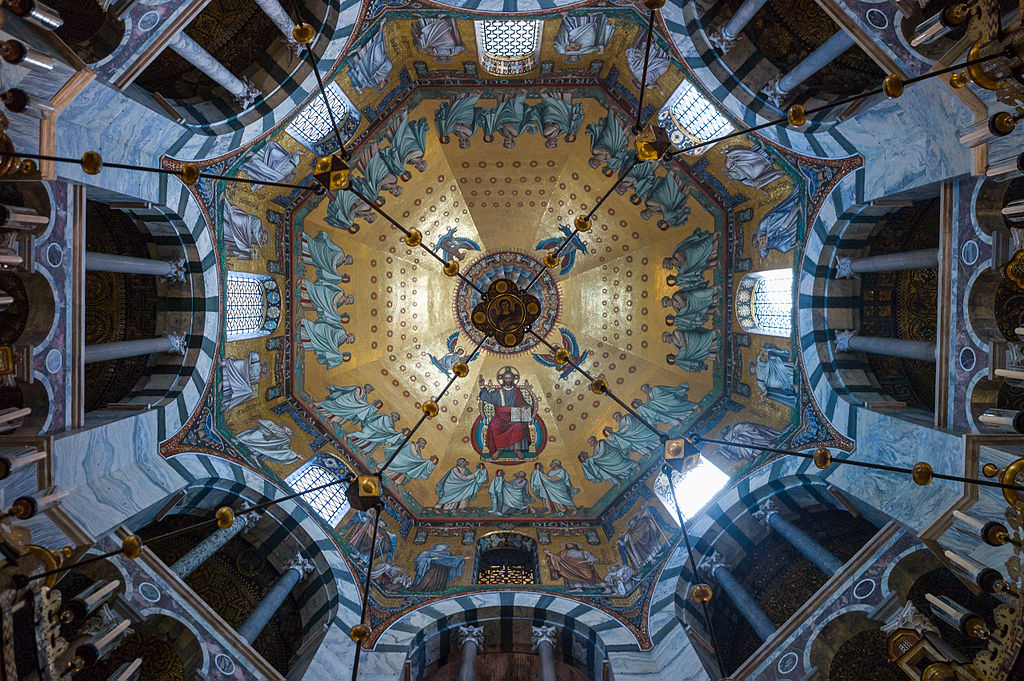
\includegraphics[height=0.6\linewidth]{../categories/media/aachen/Aachener_Dom_August_2014}
				\column{.5\textwidth}
				What a nice ceiling this building has...  				
			\end{columns}
		}
		\only<2>{
			What is Aachen cathedral?
		}
	\end{textarea}
}
	
	
\content                       
{s2-200}                     
{\secondcat}                          
{200}{     
	\begin{textarea}[]
		\only<1>{
			\begin{columns}[c] 
				\column{.5\textwidth} 
				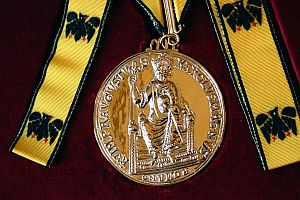
\includegraphics[height=0.5\linewidth]{../categories/media/aachen/CharlemagnePrize}
				\column{.5\textwidth}
				Parts of this building date back to Charlemagne,
				whose price is rewarded here once a year.
			\end{columns}
		}
		\only<2>{
			What is Aachen City Hall?
		}
	\end{textarea}        
}
	
	
\content           
{s2-300}                     
{\secondcat}                          
{300}{   
	\begin{textarea}[]
		\only<1>{
			\begin{columns}[c] 
				\column{.5\textwidth} 
				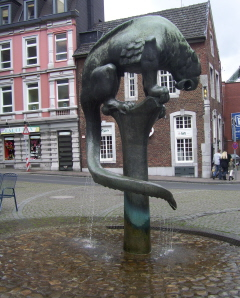
\includegraphics[height=1.0\linewidth]{../categories/media/aachen/Brunnen-am-buechel}
				\column{.5\textwidth}
				Drunk husbands used this guy as an excuse to come home late.
			\end{columns}
		}
		\only<2>{
			What is the Bahkauv?
		}
	\end{textarea}                    
}
	
	
\content                       
{s2-400}                     
{\secondcat}                          
{400}{     
	\begin{textarea}[]
		\only<1>{
			\begin{columns}[c] 
				\column{.5\textwidth} 
				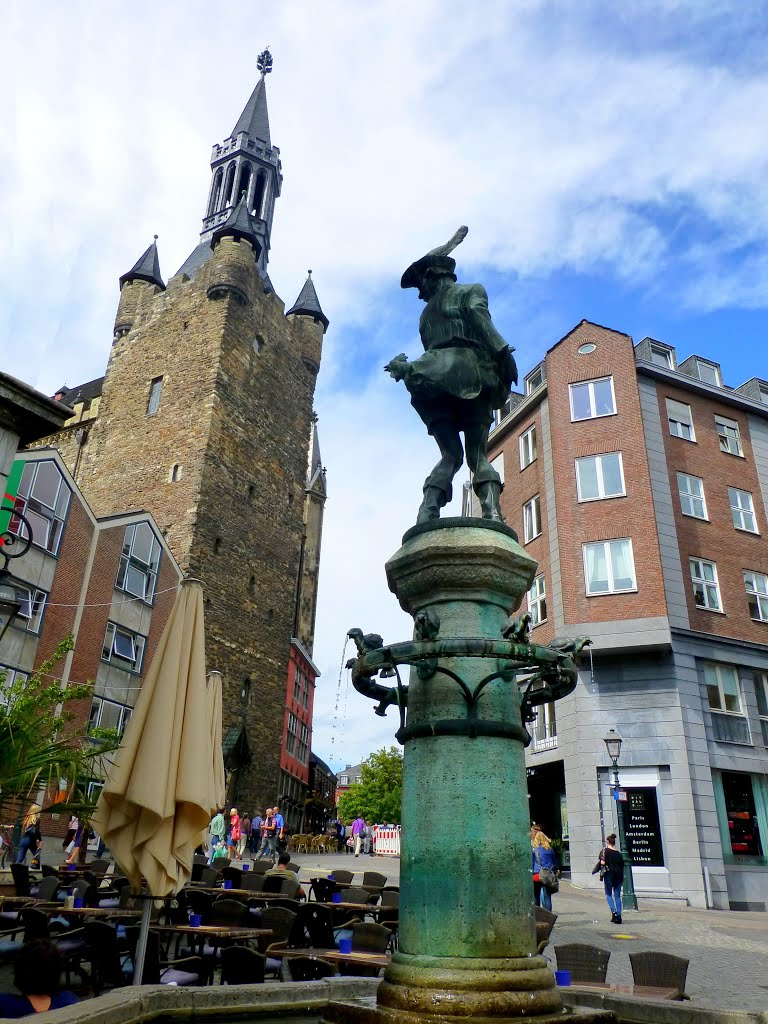
\includegraphics[height=1.0\linewidth]{../categories/media/aachen/huehnerdieb}
				\column{.5\textwidth}
				You probably don't want to see this guy on the market, especially not if you sell chicken.    
			\end{columns}
		}
		\only<2>{
			What is the H\"uhnerdieb?
		}
	\end{textarea}  
}
	
	
\content                       
{s2-500}                     
{\secondcat}                          
{500}{   
	\begin{textarea}[]
		\only<1>{
			\begin{columns}[c] 
				\column{.5\textwidth} 
				\includegraphics[height=1.0\linewidth]{../categories/media/aachen/Löwenstein_House_Aachen}
				\column{.5\textwidth}
				It is one of Aachen's oldest buildings and can be found on the market square.
			\end{columns}
									
		}
		\only<2>{
			What is L\"owenstein house?
		}
	\end{textarea} 
}
	
	
%%%%%%%%%%%%%%%%%%%%%%%%%%%%%%%%%%%%%%%%%%%%%%%%%%%%%%%%%%%%%%%%%%%%%%%%%%%%%%%
% Category 3
%%%%%%%%%%%%%%%%%%%%%%%%%%%%%%%%%%%%%%%%%%%%%%%%%%%%%%%%%%%%%%%%%%%%%%%%%%%%%%%
\content                       
{s3-100}                     
{\thirdcat}                          
{100}{    
	\begin{textarea}[]
		\only<1>{
			\begin{algorithm}[H]
				\textbf{FUNCTION} F(n)
				\begin{algorithmic}[1]
					\IF{$n \leq 1$}
					\RETURN $n$
					\ELSE
					\RETURN $F(n-1)+F(n-2)$
					\ENDIF
				\end{algorithmic}
			\end{algorithm}
		}
		\only<2>{
			What is the Fibonacci Algorithm?
		}
	\end{textarea}
}
	
	
\content                       
{s3-200}                     
{\thirdcat}                          
{200}{     
			
	\begin{textarea}[]
		\only<1>{	
			This algorithm gets you from the time domain to the frequency domain.
									
			P.S.: It's FAST!
		}
		\only<2>{
			What is the FFT.
		}
	\end{textarea}        
}
	
	
\content           
{s3-300}                     
{\thirdcat}                          
{300}{    
	\begin{textarea}[]
		\only<1>{	
			%\includemovie{5cm}{5cm}{media/code/code/Merge-sort-example-300px.gif}
			\animategraphics{80}{../categories/media/code/Merge-}{0}{211}
		}
		\only<2>{
			What is Mergesort.
		}
	\end{textarea}                   
}
	
	
\content                       
{s3-400}                     
{\thirdcat}                          
{400}{     
	\begin{textarea}[]
		\only<1>{
			\centering
			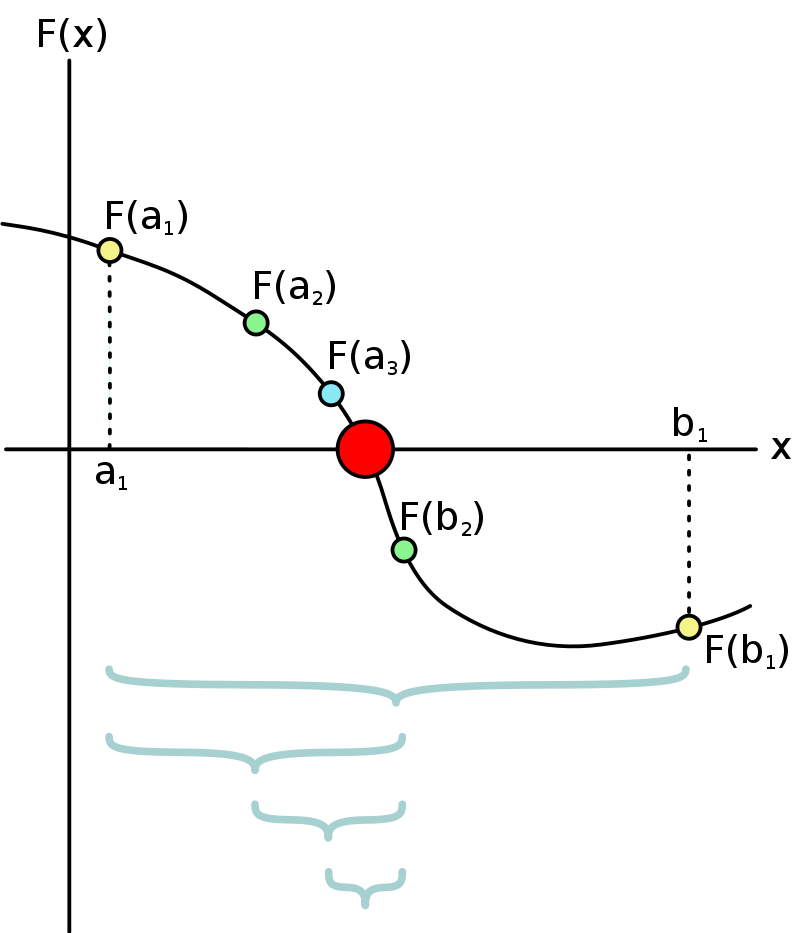
\includegraphics[height=0.5\linewidth]{../categories/media/code/800px-Bisection_method}
		}
		\only<2>{
			What is the Bisection Algorithm?
		}
	\end{textarea}  
}
	
	
\content                       
{s3-500}                     
{\thirdcat}                          
{500}{  
	\begin{textarea}[]
		\only<1>{
			\begin{algorithm}[H]
				\begin{algorithmic}[1]
					\FOR {$k = 1 \cdots n$}
					\FOR {$i = k+1 \cdots n$}
					\STATE $m := A[i, k] / A[k, k]$
					\FOR {$j = k+1 \cdots n$}
					\STATE $A[i, j]  := A[i, j] - A[k, j] * m$
					\ENDFOR
					\STATE $A[i, k]  := 0$
					\ENDFOR
					\ENDFOR
				\end{algorithmic}
			\end{algorithm}
		}
		\only<2>{
			What is the Gauss-Algorithm?
		}
	\end{textarea}  
}
	
	
%%%%%%%%%%%%%%%%%%%%%%%%%%%%%%%%%%%%%%%%%%%%%%%%%%%%%%%%%%%%%%%%%%%%%%%%%%%%%%%
% Category 4
%%%%%%%%%%%%%%%%%%%%%%%%%%%%%%%%%%%%%%%%%%%%%%%%%%%%%%%%%%%%%%%%%%%%%%%%%%%%%%%
\content                       
{s4-100}                     
{\fourthcat}                          
{100}{    
	\begin{textarea}[]
		\only<1>{
			Not only does this force pulls you towards earth, it also pulls earth towards you, isn't that cool?
		}
		\only<2>{
			What is gravitation?
		}
	\end{textarea}
}
	
	
\content                       
{s4-200}                     
{\fourthcat}                          
{200}{        
	\begin{textarea}[]
		\only<1>{
			\begin{columns}[c] 
				\column{.3\textwidth} 
				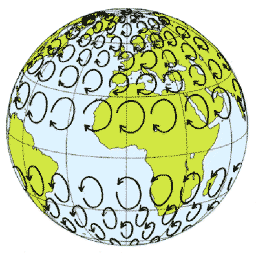
\includegraphics[height=1.0\linewidth]{../categories/media/mayTheForce/Coriolis_effect14.png}
				\column{.5\textwidth}
				On the large scale, this force influences the atmospheric behavior, even snipers and other long-distance shooters have to take it into account.
			\end{columns}
									
		}
		\only<2>{
			What is the Coriolis effect?
		}
	\end{textarea}     
}
	
	
\content           
{s4-300}                     
{\fourthcat}                          
{300}{    
	\begin{textarea}[]
		\only<1>{
			It's the force $\textbf{F}$ acting on a particle of electric charge $q$ with instantaneous velocity $\textbf{v}$, due to an external electric field $\textbf{E}$ and magnetic field $\textbf{B}$
									
			$\mathbf{F} = q(\mathbf{E} + \mathbf{v} \times \mathbf{B})$.
		}
		\only<2>{
			What is the Lorentz force?
		}
	\end{textarea}                   
}
	
	
\content                       
{s4-400}                     
{\fourthcat}                          
{400}{    
	\begin{textarea}[]
		\only<1>{
			This effect allows tennis, soccer and other ball sport player to add spin to their gaming device
		}
		\only<2>{
			What is the Magnus effect?
		}
	\end{textarea}   
}
	
	
\content                       
{s4-500}                     
{\fourthcat}                          
{500}{    
	\begin{textarea}[]
		\only<1>{
			A law of physics that describes force interacting between static electrically charged particles.
										 
			$F =k \frac{|q_1q_2|}{r^2}$.
		}
		\only<2>{
			What is the Coulomb Force?
		}
	\end{textarea}  
}
	
	
%%%%%%%%%%%%%%%%%%%%%%%%%%%%%%%%%%%%%%%%%%%%%%%%%%%%%%%%%%%%%%%%%%%%%%%%%%%%%%%
% Category 5
%%%%%%%%%%%%%%%%%%%%%%%%%%%%%%%%%%%%%%%%%%%%%%%%%%%%%%%%%%%%%%%%%%%%%%%%%%%%%%%
\content                       
{s5-100}                     
{\fifthcat}                          
{100}{ 
	\begin{textarea}[]
		\only<1>{
			\begin{align*}
			\lim_{n \to \infty} \left( 1+\frac{1}{n} \right)^n
			\end{align*}
		}
		\only<2>{
			What is $e$?
		}
	\end{textarea}   
}
	
	
\content                       
{s5-200}                     
{\fifthcat}                          
{200}{   
	\begin{textarea}[]
		\only<1>{
			\begin{align*}
			e^{i \pi}-1
			\end{align*}
		}
		\only<2>{
			What is zero?
		}
	\end{textarea}          
}
	
	
\content           
{s5-300}                     
{\fifthcat}                          
{300}{     
	\begin{textarea}[]
		\only<1>{
			\begin{align*}
			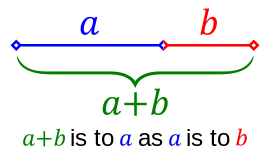
\includegraphics[width=0.5\textwidth]{../categories/media/numbers/Golden_ratio_line.png}
			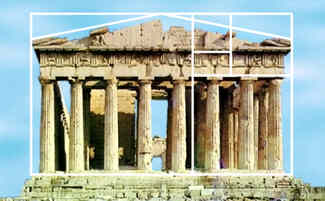
\includegraphics[width=0.5\textwidth]{../categories/media/numbers/parthenon-golden-ratio.jpg}
			\end{align*}
		}
		\only<2>{
			What is the Golden Ratio?
		}
	\end{textarea}                  
}
	
	
\content                       
{s5-400}                     
{\fifthcat}                          
{400}{ 
	\begin{textarea}[]
		\only<1>{
			\begin{align*}
			\frac{\rho v L}{\eta}
			\end{align*}
		}
		\only<2>{
			What is the Reynolds number?
		}
	\end{textarea}      
}
	
	
\content                       
{s5-500}                     
{\fifthcat}                          
{500}{   
	\begin{textarea}[]
		\only<1>{
			\begin{align*}
			42
			\end{align*}
		}
		\only<2>{
			What is the answer to the Ultimate Question of Life, the Universe, and Everything?
		}
	\end{textarea} 
}
\end{document}
